\begin{comment}
\chapter{Greedy algorithms}

\index{greedy algorithm}

A \key{greedy algorithm}
constructs a solution to the problem
by always making a choice that looks
the best at the moment.
A greedy algorithm never takes back
its choices, but directly constructs
the final solution.
For this reason, greedy algorithms
are usually very efficient.

The difficulty in designing greedy algorithms
is to find a greedy strategy
that always produces an optimal solution
to the problem.
The locally optimal choices in a greedy
algorithm should also be globally optimal.
It is often difficult to argue that
a greedy algorithm works.
\end{comment}


\chapter{貪欲アルゴリズム}

\index{greedy algorithm}
\index{貪欲アルゴリズム}

\key{貪欲アルゴリズム}は、そのつど最良に見える手を選択していく
形で解法を構成する手法である。

貪欲アルゴリズムは選択結果を巻き戻すことはせず、
直接最終的な解を構成する。
そのため、貪欲アルゴリズムは通常非常に効率的である。

貪欲アルゴリズムの設計の難しさは、問題に対し必ず最適化を
生成できるような貪欲な戦略を探すところにある。
局所的に最適な選択が、全体でも最適でなければならない。
そのため、貪欲解法で正答できると判断するのはしばしば
難しい場合がある。

\begin{comment}
\section{Coin problem}

As a first example, we consider a problem
where we are given a set of coins
and our task is to form a sum of money $x$
using the coins.
The values of the coins are
$\texttt{coins}=\{c_1,c_2,\ldots,c_k\}$,
and each coin can be used as many times we want.
What is the minimum number of coins needed?

For example, if the coins are the euro coins (in cents)
\[\{1,2,5,10,20,50,100,200\}\]
and $x=520$,
we need at least four coins.
The optimal solution is to select coins
$200+200+100+20$ whose sum is 520.
\end{comment}

\section{コインの問題}

最初の例として、コインの集合が与えられたとき、
和が$n$となるようなコインの部分集合を求める問題を考えよう。
それぞれのコインの価値は$\texttt{coins}=\{c_1,c_2,\ldots,c_k\}$であるとし、
それぞれのコインは好きなだけ利用できるとする。
部分集合を構成する際最小の枚数はいくつになるだろうか?

例えば、ユーロにおけるコインの金額の種類は\[\{1,2,5,10,20,50,100,200\}\]であり、
和$x$が$520$となるケースでは、コインは最小4枚必要である。
最適な解はコインを$200+200+100+20 = 520$となるように選択することである。

\begin{comment}
\subsubsection{Greedy algorithm}

A simple greedy algorithm to the problem
always selects the largest possible coin,
until the required sum of money has been constructed.
This algorithm works in the example case,
because we first select two 200 cent coins,
then one 100 cent coin and finally one 20 cent coin.
But does this algorithm always work?

It turns out that if the coins are the euro coins,
the greedy algorithm \emph{always} works, i.e.,
it always produces a solution with the fewest
possible number of coins.
The correctness of the algorithm can be
shown as follows:
\end{comment}

\subsubsection{貪欲アルゴリズム}

この問題に対するシンプルな貪欲アルゴリズムは、
和が$x$に達するまで、できるだけ大きな金額のコインを使っていくことである。
このアルゴリズムは上記の例ではうまく動作する。
まず200セントのコインを2枚選択し、100セントのコインを1枚選択して
最後に20セントのコインを選択すればよい。
しかしこのアルゴリズムは常に有効なのだろうか?

コインの種類がユーロと同じであれば、この貪欲アルゴリズムは
\emph{常に}正解を返す。
つまり最小のコイン枚数の解を得ることができる。
このアルゴリズムの正しさは下記の通り示すことができる:

\begin{comment}
First, each coin 1, 5, 10, 50 and 100 appears
at most once in an optimal solution,
because if the
solution would contain two such coins,
we could replace them by one coin and
obtain a better solution.
For example, if the solution would contain
coins $5+5$, we could replace them by coin $10$.

In the same way, coins 2 and 20 appear
at most twice in an optimal solution,
because we could replace
coins $2+2+2$ by coins $5+1$ and
coins $20+20+20$ by coins $50+10$.
Moreover, an optimal solution cannot contain
coins $2+2+1$ or $20+20+10$,
because we could replace them by coins $5$ and $50$.
\end{comment}

まず、1,5,10,50,100のコインは最適解において高々1枚しか
選択しえない。というのも、これらのコインが2枚あるのであれば、
より金額の高い1枚と置き換えることでより良い解を得られるからである。
例えば、もし解が$5+5$を含むのであれば、$10$のコインに置き換えることができる。

同様に、2,20のコインも最適解では高々2枚までしか含まれない。
というのも、$2+2+2$の構成は$5+1$に、$20+20+20$の構成は
$50+10$に置き換えられるからである。
さらに、最適解は$2+2+1$や$20+20+10$という構成も持ちえない。
これらは$5$や$50$のコイン1枚に置き換えられるためである。

\begin{comment}
Using these observations,
we can show for each coin $x$ that
it is not possible to optimally construct
a sum $x$ or any larger sum by only using coins
that are smaller than $x$.
For example, if $x=100$, the largest optimal
sum using the smaller coins is  $50+20+20+5+2+2=99$.
Thus, the greedy algorithm that always selects
the largest coin produces the optimal solution.

This example shows that it can be difficult
to argue that a greedy algorithm works,
even if the algorithm itself is simple.
\end{comment}

これらの考察より、
各コイン$x$に対して、$x$を用いずに和が$x$以上となる
組み合わせの最適化を構成できないことがわかる。
例えば、$x=100$を例にすると、これより小さい価値のコインで
表せる最適解が最大枚数となるケースは$50+20+20+5+2+2=99$となる。
そのため、常に最大価値のコインを選択する貪欲アルゴリズムは
最適解を生成できる。

この例は、アルゴリズム自体は単純でもそれが最適であることを
示すのが比較的難しいことを示す好例である。

\begin{comment}
\subsubsection{General case}

In the general case, the coin set can contain any coins
and the greedy algorithm \emph{does not} necessarily produce
an optimal solution.

We can prove that a greedy algorithm does not work
by showing a counterexample
where the algorithm gives a wrong answer.
In this problem we can easily find a counterexample:
if the coins are $\{1,3,4\}$ and the target sum
is 6, the greedy algorithm produces the solution
$4+1+1$ while the optimal solution is $3+3$.

It is not known if the general coin problem
can be solved using any greedy algorithm\footnote{However, it is possible
to \emph{check} in polynomial time
if the greedy algorithm presented in this chapter works for
a given set of coins \cite{pea05}.}.
However, as we will see in Chapter 7,
in some cases,
the general problem can be efficiently
solved using a dynamic
programming algorithm that always gives the
correct answer.
\end{comment}

\subsubsection{一般的な例}

コインンの組み合わせを任意に設定できる場合において、
この貪欲アルゴリズムは最適解を生成できるとは\emph{限らない}。

これは前述の貪欲アルゴリズムが非最適解を返す反例を持って
示すことができる。
コインの種類が$\{1,3,4\}$で和を6としたい場合、
最適解は$3+3$だが、貪欲アルゴリズムでは$4+1+1$となってしまう。

この一般的な例が貪欲解法で解けるかどうかは分かっていない
\footnote{しかし、前述の貪欲解法で解けるコイン種別かどうかを多項式時間で
判定することはできる\cite{pea05}。}。
しかし、7章で例を示す通り、動的計画法でこの問題は効率よく解くことができる。

\begin{comment}
\section{Scheduling}

Many scheduling problems can be solved
using greedy algorithms.
A classic problem is as follows:
Given $n$ events with their starting and ending
times, find a schedule
that includes as many events as possible.
It is not possible to select an event partially.
For example, consider the following events:
\begin{center}
\begin{tabular}{lll}
event & starting time & ending time \\
\hline
$A$ & 1 & 3 \\
$B$ & 2 & 5 \\
$C$ & 3 & 9 \\
$D$ & 6 & 8 \\
\end{tabular}
\end{center}
\end{comment}

\section{スケジューリング}

多くのスケジューリング問題は貪欲アルゴリズムで解くことができる。
ここで古典的問題を考えよう。
$n$個のイベントがあり、開始時間と終了時間が与えられる。
最適にイベントをスケジューリングしたとき、最大でいくつのイベントを
含むことができるか。
ただしイベントの開催時間の一部だけ参加するということはできない。

例えば以下のイベント例を考える:
\begin{center}
\begin{tabular}{lll}
イベント & 開始時間 & 終了時間 \\
\hline
$A$ & 1 & 3 \\
$B$ & 2 & 5 \\
$C$ & 3 & 9 \\
$D$ & 6 & 8 \\
\end{tabular}
\end{center}

\begin{comment}
In this case the maximum number of events is two.
For example, we can select events $B$ and $D$
as follows:
\end{comment}

この例ではイベントの最大数は2である。
例えば下記のようにイベント$B$と$D$を選ぶことができる:
\begin{center}
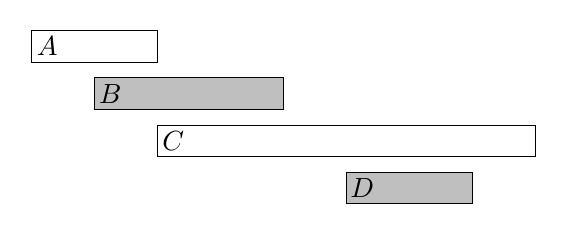
\begin{tikzpicture}[scale=.4]
  \begin{scope}
    \draw (2, 0) rectangle (6, -1);
    \draw[fill=lightgray] (4, -1.5) rectangle (10, -2.5);
    \draw (6, -3) rectangle (18, -4);
    \draw[fill=lightgray] (12, -4.5) rectangle (16, -5.5);
    \node at (2.5,-0.5) {$A$};
    \node at (4.5,-2) {$B$};
    \node at (6.5,-3.5) {$C$};
    \node at (12.5,-5) {$D$};
  \end{scope}
\end{tikzpicture}
\end{center}

\begin{comment}
この問題について、色々貪欲アルゴリズムを考えることはできるだろうが、
どんなケースにもうまく解答できるのはどんなアルゴリズムだろうか?
\end{comment}

\begin{comment}
\subsubsection*{Algorithm 1}

The first idea is to select as \emph{short}
events as possible.
In the example case this algorithm
selects the following events:
\end{comment}

\subsubsection*{アルゴリズム 1}

最初のアイデアは、\emph{短い}イベントをできるだけ選んでいく方法である。
サンプルケースでは、このアルゴリズムは以下のようにイベントを選ぶ:

\begin{center}
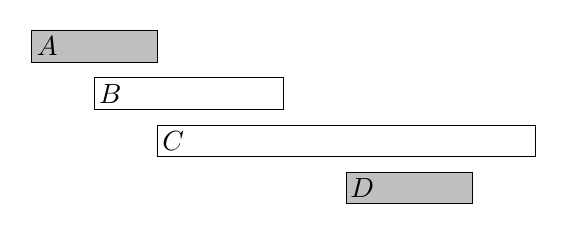
\begin{tikzpicture}[scale=.4]
  \begin{scope}
    \draw[fill=lightgray] (2, 0) rectangle (6, -1);
    \draw (4, -1.5) rectangle (10, -2.5);
    \draw (6, -3) rectangle (18, -4);
    \draw[fill=lightgray] (12, -4.5) rectangle (16, -5.5);
    \node at (2.5,-0.5) {$A$};
    \node at (4.5,-2) {$B$};
    \node at (6.5,-3.5) {$C$};
    \node at (12.5,-5) {$D$};
  \end{scope}
\end{tikzpicture}
\end{center}

\begin{comment}
However, selecting short events is not always
a correct strategy. For example, the algorithm fails
in the following case:
\end{comment}

しかし、短いイベントを選ぶ方法は常に正解とは限らない。
例えば次の例では正解を得られない:
\begin{center}
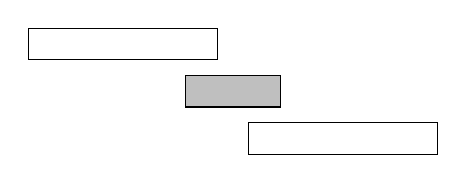
\begin{tikzpicture}[scale=.4]
  \begin{scope}
    \draw (1, 0) rectangle (7, -1);
    \draw[fill=lightgray] (6, -1.5) rectangle (9, -2.5);
    \draw (8, -3) rectangle (14, -4);
  \end{scope}
\end{tikzpicture}
\end{center}

\begin{comment}
If we select the short event, we can only select one event.
However, it would be possible to select both long events.
\end{comment}

この例では、短いイベントを選ぶと1つしかイベントを選択できない。
しかし明らかに長いイベントを2つ選ぶ方が正解である。

\begin{comment}
\subsubsection*{Algorithm 2}

Another idea is to always select the next possible
event that \emph{begins} as \emph{early} as possible.
This algorithm selects the following events:
\end{comment}

\subsubsection*{アルゴリズム 2}

次のアイデアは、\emph{開始時間}ができるだけ\emph{早いもの}を
できる限り選んでいく方法である。
このアルゴリズムでは以下のようにイベントが選択される:

\begin{center}
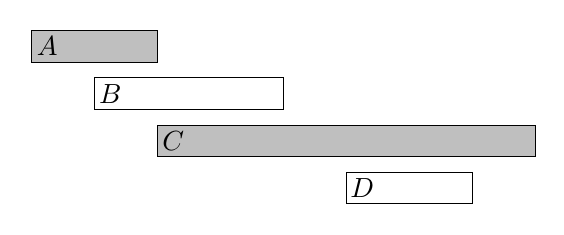
\begin{tikzpicture}[scale=.4]
  \begin{scope}
    \draw[fill=lightgray] (2, 0) rectangle (6, -1);
    \draw (4, -1.5) rectangle (10, -2.5);
    \draw[fill=lightgray] (6, -3) rectangle (18, -4);
    \draw (12, -4.5) rectangle (16, -5.5);
    \node at (2.5,-0.5) {$A$};
    \node at (4.5,-2) {$B$};
    \node at (6.5,-3.5) {$C$};
    \node at (12.5,-5) {$D$};
  \end{scope}
\end{tikzpicture}
\end{center}

\begin{comment}
However, we can find a counterexample
also for this algorithm.
For example, in the following case,
the algorithm only selects one event:
\end{comment}

しかし、このアルゴリズムに対しても反例が存在する。
以下の例では、このアルゴリズムでは1つしかイベントを選択できない:

\begin{center}
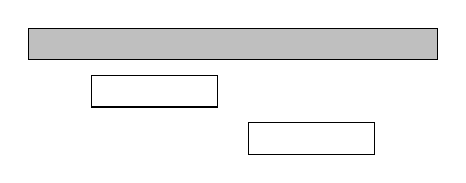
\begin{tikzpicture}[scale=.4]
  \begin{scope}
    \draw[fill=lightgray] (1, 0) rectangle (14, -1);
    \draw (3, -1.5) rectangle (7, -2.5);
    \draw (8, -3) rectangle (12, -4);
  \end{scope}
\end{tikzpicture}
\end{center}

もし最初のイベントを選ぶと、それ以上他のイベントを選べない。
しかし、最初のイベントの選択をあきらめれば、残り2つの
イベントを選ぶことができる。

\begin{comment}
\subsubsection*{Algorithm 3}

The third idea is to always select the next
possible event that \emph{ends} as \emph{early} as possible.
This algorithm selects the following events: 
\end{comment}

\subsubsection*{アルゴリズム 3}

3つ目のアルゴリズムは、\emph{終了時間}ができるだけ\emph{早いもの}を
できる限り選んでいく方法である。
このアルゴリズムでは以下のようにイベントを選択する:
\begin{center}
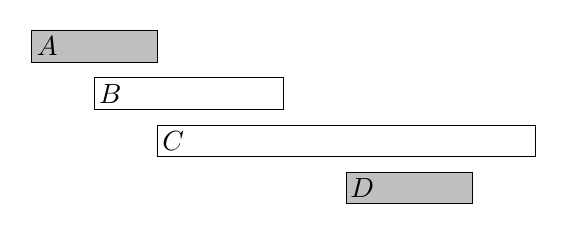
\begin{tikzpicture}[scale=.4]
  \begin{scope}
    \draw[fill=lightgray] (2, 0) rectangle (6, -1);
    \draw (4, -1.5) rectangle (10, -2.5);
    \draw (6, -3) rectangle (18, -4);
    \draw[fill=lightgray] (12, -4.5) rectangle (16, -5.5);
    \node at (2.5,-0.5) {$A$};
    \node at (4.5,-2) {$B$};
    \node at (6.5,-3.5) {$C$};
    \node at (12.5,-5) {$D$};
  \end{scope}
\end{tikzpicture}
\end{center}

\begin{comment}
It turns out that this algorithm
\emph{always} produces an optimal solution.
The reason for this is that it is always an optimal choice
to first select an event that ends
as early as possible.
After this, it is an optimal choice
to select the next event
using the same strategy, etc.,
until we cannot select any more events.

One way to argue that the algorithm works
is to consider
what happens if we first select an event
that ends later than the event that ends
as early as possible.
Now, we will have at most an equal number of
choices how we can select the next event.
Hence, selecting an event that ends later
can never yield a better solution,
and the greedy algorithm is correct.
\end{comment}

このアルゴリズムは\emph{常に}最適解を返すことがわかる。
その理由は、終了時間の早いイベントを最初に選ぶことが
常に最適な選択であるからである。
そのイベントの後は、同様の手順で次のイベントを最適に
選択していくことを、それ以上イベントが選べなくなるまで繰り返す。

このアルゴリズムがうまく動くことを示す1つの方法は、
終了時間が早くないイベントを選んだ時何が起きるかを
考えることである。
その場合、以後どれだけ最適な選び方をしても、
最初のイベントで終了時間が早いものを選んだ場合と
せいぜい同数にしかならない。
よって、終了時間の遅いものを選ぶことがより良い解と
なることはなく、この貪欲アルゴリズムは正しい。


\begin{comment}
\section{Tasks and deadlines}

Let us now consider a problem where
we are given $n$ tasks with durations and deadlines
and our task is to choose an order to perform the tasks.
For each task, we earn $d-x$ points
where $d$ is the task's deadline
and $x$ is the moment when we finish the task.
What is the largest possible total score
we can obtain?

For example, suppose that the tasks are as follows:
\begin{center}
\begin{tabular}{lll}
task & duration & deadline \\
\hline
$A$ & 4 & 2 \\
$B$ & 3 & 5 \\
$C$ & 2 & 7 \\
$D$ & 4 & 5 \\
\end{tabular}
\end{center}
In this case, an optimal schedule for the tasks
is as follows:
\end{comment}

\section{タスクと締切}

次に、別の問題を考えよう。
$n$個のタスクについて、実行時間と締切時刻が与えられる。
これらのタスクを処理する順番を考えよう。
各タスクについて、締切時刻を$d$、タスクを終了した時刻を$x$とすると、
$d-x$ポイントの点を得られるものとする。
総得点の最大値はどうなるだろうか?

例えば、タスクが以下の通りだとする:
\begin{center}
\begin{tabular}{lll}
タスク名 & 実行時間 & 締切時刻 \\
\hline
$A$ & 4 & 2 \\
$B$ & 3 & 5 \\
$C$ & 2 & 7 \\
$D$ & 4 & 5 \\
\end{tabular}
\end{center}

この例では、最適なスケジュールは以下のようになる:

\begin{center}
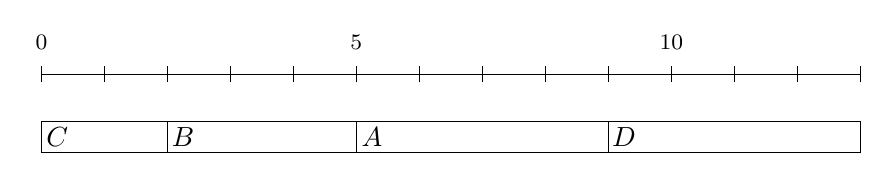
\begin{tikzpicture}[scale=.4]
  \begin{scope}
    \draw (0, 0) rectangle (4, -1);
    \draw (4, 0) rectangle (10, -1);
    \draw (10, 0) rectangle (18, -1);
    \draw (18, 0) rectangle (26, -1);
    \node at (0.5,-0.5) {$C$};
    \node at (4.5,-0.5) {$B$};
    \node at (10.5,-0.5) {$A$};
    \node at (18.5,-0.5) {$D$};

    \draw (0,1.5) -- (26,1.5);
    \foreach \i in {0,2,...,26}
    {
        \draw (\i,1.25) -- (\i,1.75);
    }
    \footnotesize
    \node at (0,2.5) {0};
    \node at (10,2.5) {5};
    \node at (20,2.5) {10};

  \end{scope}
\end{tikzpicture}
\end{center}

\begin{comment}
In this solution, $C$ yields 5 points,
$B$ yields 0 points, $A$ yields $-7$ points
and $D$ yields $-8$ points,
so the total score is $-10$.

Surprisingly, the optimal solution to the problem
does not depend on the deadlines at all,
but a correct greedy strategy is to simply
perform the tasks \emph{sorted by their durations}
in increasing order.
The reason for this is that if we ever perform
two tasks one after another such that the first task
takes longer than the second task,
we can obtain a better solution if we swap the tasks.
For example, consider the following schedule:
\end{comment}

この回答では、$C$で5ポイント、$B$で0ポイント、
$A$で$-7$ポイント、$D$で$-10$ポイント得ることができ、
総得点は$-10$ポイントとなる。

驚くことに、この問題の最適解は締切時刻には全く関係ない。
正しく動作する貪欲な戦略は、単にタスクを\emph{実行時間で昇順に
ソートする}ことである。
その理由は、2つの連続するタスクにおいて前者が後者より
実行時間が長い場合、それらを交換することでより良い解を
得られるためである。
例えば、以下のスケジュールを考えよう:
\begin{center}
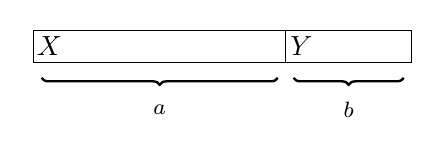
\begin{tikzpicture}[scale=.4]
  \begin{scope}
    \draw (0, 0) rectangle (8, -1);
    \draw (8, 0) rectangle (12, -1);
    \node at (0.5,-0.5) {$X$};
    \node at (8.5,-0.5) {$Y$};

\draw [decoration={brace}, decorate, line width=0.3mm] (7.75,-1.5) -- (0.25,-1.5);
\draw [decoration={brace}, decorate, line width=0.3mm] (11.75,-1.5) -- (8.25,-1.5);

\footnotesize
\node at (4,-2.5) {$a$};
\node at (10,-2.5) {$b$};

  \end{scope}
\end{tikzpicture}
\end{center}

\begin{comment}
Here $a>b$, so we should swap the tasks:
\end{comment}

ここで$a>b$なので、両者は交換するべきである:
\begin{center}
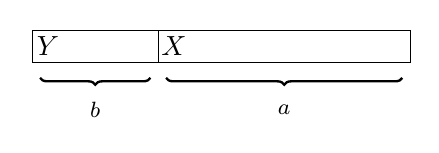
\begin{tikzpicture}[scale=.4]
  \begin{scope}
    \draw (0, 0) rectangle (4, -1);
    \draw (4, 0) rectangle (12, -1);
    \node at (0.5,-0.5) {$Y$};
    \node at (4.5,-0.5) {$X$};

\draw [decoration={brace}, decorate, line width=0.3mm] (3.75,-1.5) -- (0.25,-1.5);
\draw [decoration={brace}, decorate, line width=0.3mm] (11.75,-1.5) -- (4.25,-1.5);

\footnotesize
\node at (2,-2.5) {$b$};
\node at (8,-2.5) {$a$};

  \end{scope}
\end{tikzpicture}
\end{center}

\begin{comment}
Now $X$ gives $b$ points less and $Y$ gives $a$ points more,
so the total score increases by $a-b > 0$.
In an optimal solution,
for any two consecutive tasks,
it must hold that the shorter task comes
before the longer task.
Thus, the tasks must be performed
sorted by their durations.
\end{comment}

ここでタスク$X$により得られるポイントは$b$減少し、
タスク$Y$により得られるポイントは$a$増加する。
よって総得点は$a-b > 0$だけ増加する。
最適解では、2つの連続するタスクでは常に先行するタスクには
実行時間が短いほうが割り当てられる。
よって、タスクは実行時間で昇順ソートした順で処理されなければならない。

\begin{comment}
\section{Minimizing sums}

We next consider a problem where
we are given $n$ numbers $a_1,a_2,\ldots,a_n$
and our task is to find a value $x$
that minimizes the sum
\[|a_1-x|^c+|a_2-x|^c+\cdots+|a_n-x|^c.\]
We focus on the cases $c=1$ and $c=2$.
\end{comment}

\section{和の最小化}

次の問題として、$n$個の数値$a_1,a_2,\ldots,a_n$が与えられたとき、
和\[|a_1-x|^c+|a_2-x|^c+\cdots+|a_n-x|^c.\]
を最小化するような数$x$を求める問題を考えてみよう。
ここでは$c=1$と$c=2$の場合のみ考える。

\begin{comment}
\subsubsection{Case $c=1$}

In this case, we should minimize the sum
\[|a_1-x|+|a_2-x|+\cdots+|a_n-x|.\]
For example, if the numbers are $[1,2,9,2,6]$,
the best solution is to select $x=2$
which produces the sum
\[
|1-2|+|2-2|+|9-2|+|2-2|+|6-2|=12.
\]
In the general case, the best choice for $x$
is the \textit{median} of the numbers,
i.e., the middle number after sorting.
For example, the list $[1,2,9,2,6]$
becomes $[1,2,2,6,9]$ after sorting,
so the median is 2.
\end{comment}

\subsubsection{$c=1$の場合}

この場合、以下の和を最小化する問題となる。
\[|a_1-x|+|a_2-x|+\cdots+|a_n-x|.\]
例えば、入力の数が$[1,2,9,2,6]$であれば、
最適解は$x=2$であり、その時の和は下記のとおりとなる。
\[
|1-2|+|2-2|+|9-2|+|2-2|+|6-2|=12.
\]
一般に、$x$の最適値は数値群の\textit{中央値}
(注:要素をソートした後の中央の値)となる。
例えば、入力の数値群$[1,2,9,2,6]$はソート後
$[1,2,2,6,9]$となるので、中央値は2である。

\begin{comment}
The median is an optimal choice,
because if $x$ is smaller than the median,
the sum becomes smaller by increasing $x$,
and if $x$ is larger then the median,
the sum becomes smaller by decreasing $x$.
Hence, the optimal solution is that $x$
is the median.
If $n$ is even and there are two medians,
both medians and all values between them
are optimal choices.
\end{comment}

中央値が最適値となるのは、
もし$x$が中央値より小さい場合、和は$x$を
大きくする毎に小さくなり、逆に$x$が中央値より大きいならば、
和は$x$をへらほど小さくなる。
よって最適解は$x$を中央値とすることである。
$n$が偶数の場合中央値は2つあるが、
その場合両方の値、および両者の間にあるあらゆる数が
最適解となる。

\begin{comment}
\subsubsection{Case $c=2$}

In this case, we should minimize the sum
\[(a_1-x)^2+(a_2-x)^2+\cdots+(a_n-x)^2.\]
For example, if the numbers are $[1,2,9,2,6]$,
the best solution is to select $x=4$
which produces the sum
\[
(1-4)^2+(2-4)^2+(9-4)^2+(2-4)^2+(6-4)^2=46.
\]
In the general case, the best choice for $x$
is the \emph{average} of the numbers.
In the example the average is $(1+2+9+2+6)/5=4$.
This result can be derived by presenting
the sum as follows:
\[
nx^2 - 2x(a_1+a_2+\cdots+a_n) + (a_1^2+a_2^2+\cdots+a_n^2)
\]
The last part does not depend on $x$,
so we can ignore it.
The remaining parts form a function
$nx^2-2xs$ where $s=a_1+a_2+\cdots+a_n$.
This is a parabola opening upwards
with roots $x=0$ and $x=2s/n$,
and the minimum value is the average
of the roots $x=s/n$, i.e.,
the average of the numbers $a_1,a_2,\ldots,a_n$.
\end{comment}

\subsubsection{$c=2$の場合}

この場合、以下の和を最小化する問題となる。
\[(a_1-x)^2+(a_2-x)^2+\cdots+(a_n-x)^2.\]
例えば、入力値が$[1,2,9,2,6]$の場合、
$x=4$が最適解であり、その時の和は下記のようになる。
\[
(1-4)^2+(2-4)^2+(9-4)^2+(2-4)^2+(6-4)^2=46.
\]
一般に、$x$の最適解は入力値の\emph{平均値}となる。
この例では平均値は$(1+2+9+2+6)/5=4$である。
この結果は、和を以下のように表現するとわかる:
\[
nx^2 - 2x(a_1+a_2+\cdots+a_n) + (a_1^2+a_2^2+\cdots+a_n^2)
\]
最後の項は$x$の値によらないので無視できる。
残りの項は、$s=a_1+a_2+\cdots+a_n$とおくと
$nx^2-2xs$と表せる。
これは上に開いた放物線で、$x=0$と$x=2s/n$が根となる。
そして最小値は$x=s/n$のときに得られるが、
これは先ほど計算した平均値そのものである。

\begin{comment}
\section{Data compression}

\index{data compression}
\index{binary code}
\index{codeword}

A \key{binary code} assigns for each character
of a string a \key{codeword} that consists of bits.
We can \emph{compress} the string using the binary code
by replacing each character by the
corresponding codeword.
For example, the following binary code
assigns codewords for characters
\texttt{A}–\texttt{D}:
\begin{center}
\begin{tabular}{rr}
character & codeword \\
\hline
\texttt{A} & 00 \\
\texttt{B} & 01 \\
\texttt{C} & 10 \\
\texttt{D} & 11 \\
\end{tabular}
\end{center}
\end{comment}

\section{データ圧縮}

\index{data compression}
\index{binary code}
\index{codeword}

\index{データ圧縮}
\index{バイナリコード}
\index{符号表}

\key{バイナリコード}は 文字列を構成する個々の文字に、
ビット列からなる\key{符号表}を割り当てる。
ここで、文字列の個々の文字を符号表を用いて対応する
バイナリコードに置き換えることで、文字列を圧縮できる。
例えば、文字\texttt{A}–\texttt{D}に対し
以下のようなバイナリコードの対応表があるとする:
\begin{center}
\begin{tabular}{rr}
文字 & 符号 \\
\hline
\texttt{A} & 00 \\
\texttt{B} & 01 \\
\texttt{C} & 10 \\
\texttt{D} & 11 \\
\end{tabular}
\end{center}

\begin{comment}
This is a \key{constant-length} code
which means that the length of each
codeword is the same.
For example, we can compress the string
\texttt{AABACDACA} as follows:
\[00\,00\,01\,00\,10\,11\,00\,10\,00\]
Using this code, the length of the compressed
string is 18 bits.
However, we can compress the string better
if we use a \key{variable-length} code
where codewords may have different lengths.
Then we can give short codewords for
characters that appear often
and long codewords for characters
that appear rarely.
It turns out that an \key{optimal} code
for the above string is as follows:
\begin{center}
\begin{tabular}{rr}
character & codeword \\
\hline
\texttt{A} & 0 \\
\texttt{B} & 110 \\
\texttt{C} & 10 \\
\texttt{D} & 111 \\
\end{tabular}
\end{center}
\end{comment}

各符号長は等しいため、これは\key{固定長}の符号と
いうことになる。
例えば、文字列\texttt{AABACDACA}は符号表により
圧縮すると\[00\,00\,01\,00\,10\,11\,00\,10\,00\]となる。
この符号表では、圧縮後の文字列は18ビットとなる。
しかし、この文字列は各符号の長さにばらつきを許容する
\key{可変長}の符号を用いることでより良く圧縮できる。
頻繁に現れる文字に短い符号、稀にしか現れない文字に
長い符号を割り当ててみる。
すると、上記文字列に対応する\key{最適な}符号表は
このようになる:
\begin{center}
\begin{tabular}{rr}
文字 & 符号 \\
\hline
\texttt{A} & 0 \\
\texttt{B} & 110 \\
\texttt{C} & 10 \\
\texttt{D} & 111 \\
\end{tabular}
\end{center}

\begin{comment}
An optimal code produces a compressed string
that is as short as possible.
In this case, the compressed string using
the optimal code is
\[0\,0\,110\,0\,10\,111\,0\,10\,0,\]
so only 15 bits are needed instead of 18 bits.
Thus, thanks to a better code it was possible to
save 3 bits in the compressed string.
\end{comment}

最適な符号表では、文字列をできるだけ短く圧縮する。
この例では、圧縮後の文字列は
\[0\,0\,110\,0\,10\,111\,0\,10\,0,\]
であり、固定長の符号表では18ビットだった文字列が
こちらではたった15ビットで済んでいる。
つまり、より良い符号表により圧縮後の文字列が
3ビット節約できている。

\begin{comment}
We require that no codeword
is a prefix of another codeword.
For example, it is not allowed that a code
would contain both codewords 10
and 1011.
The reason for this is that we want
to be able to generate the original string
from the compressed string.
If a codeword could be a prefix of another codeword,
this would not always be possible.
For example, the following code is \emph{not} valid:
\begin{center}
\begin{tabular}{rr}
character & codeword \\
\hline
\texttt{A} & 10 \\
\texttt{B} & 11 \\
\texttt{C} & 1011 \\
\texttt{D} & 111 \\
\end{tabular}
\end{center}
Using this code, it would not be possible to know
if the compressed string 1011 corresponds to
the string \texttt{AB} or the string \texttt{C}.
\end{comment}

この符号表において、ある符号が他の符号のprefixになっていてはならない。
例えば、符号表に10と1011が混在してはならない。
その理由は、圧縮後の文字列から元の文字列を復元可能で
なければならないためである。
もしある符号が他の符号のprefixだと、復元が正しく
行えない場合が生じてしまう。
例えば、以下の符号表は\emph{不正}である:
\begin{center}
\begin{tabular}{rr}
文字 & 符号 \\
\hline
\texttt{A} & 10 \\
\texttt{B} & 11 \\
\texttt{C} & 1011 \\
\texttt{D} & 111 \\
\end{tabular}
\end{center}
この符号表では、圧縮後の文字列 1011から、
元の文字列が\texttt{AB}と\texttt{C}のどちらであるか
判断できない。

\begin{comment}
\index{Huffman coding}

\subsubsection{Huffman coding}

\key{Huffman coding}\footnote{D. A. Huffman discovered this method
when solving a university course assignment
and published the algorithm in 1952 \cite{huf52}.} is a greedy algorithm
that constructs an optimal code for
compressing a given string.
The algorithm builds a binary tree
based on the frequencies of the characters
in the string,
and each character's codeword can be read
by following a path from the root to
the corresponding node.
A move to the left corresponds to bit 0,
and a move to the right corresponds to bit 1.
\end{comment}

\index{ハフマン符号}

\subsubsection{ハフマン符号}

\key{ハフマン符号}\footnote{D. A. Huffmanはこの手法を大学の授業の時間割を
考えている時に発明し、1952にこのアルゴリズムを発表した \cite{huf52}。}
は文字列に対し最適な符号表を生成する貪欲アルゴリズムである。
このアルゴリズムは、文字列中の文字の登場頻度に応じ二分木を作る。
そして各文字の符号は根から各文字に対応する頂点までのパスに対応付けられる。
木を辿る過程で、二分木の左の子を辿るとき0、右の子を辿るとき1に対応付けられる。

\begin{comment}
Initially, each character of the string is
represented by a node whose weight is the
number of times the character occurs in the string.
Then at each step two nodes with minimum weights
are combined by creating
a new node whose weight is the sum of the weights
of the original nodes.
The process continues until all nodes have been combined.

Next we will see how Huffman coding creates
the optimal code for the string
\texttt{AABACDACA}.
Initially, there are four nodes that correspond
to the characters of the string:
\end{comment}

初期状態では、文字列中の各文字は単独の頂点を無し、
その重さは文字列中の登場回数とする。
1ステップごとに、重さが最少の頂点2つを選び、
それら2つを子頂点とする親頂点を生成する。
親頂点の重さは、子頂点の重さの和である。
この処理を全頂点が連結するまで繰り返す。

以下、ハフマン符号により文字列\texttt{AABACDACA}の
符号表を作る過程を見ていこう。
初期状態では、文字列中の文字に対応し
以下の通り4つの頂点がある:.

\begin{center}
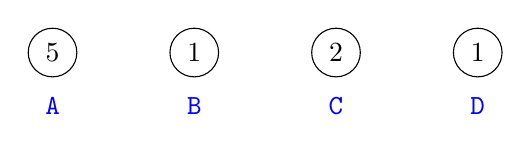
\begin{tikzpicture}[scale=0.9]
\node[draw, circle] (1) at (0,0) {$5$};
\node[draw, circle] (2) at (2,0) {$1$};
\node[draw, circle] (3) at (4,0) {$2$};
\node[draw, circle] (4) at (6,0) {$1$};

\node[color=blue] at (0,-0.75) {\texttt{A}};
\node[color=blue] at (2,-0.75) {\texttt{B}};
\node[color=blue] at (4,-0.75) {\texttt{C}};
\node[color=blue] at (6,-0.75) {\texttt{D}};

%\path[draw,thick,-] (4) -- (5);
\end{tikzpicture}
\end{center}

\begin{comment}
The node that represents character \texttt{A}
has weight 5 because character \texttt{A}
appears 5 times in the string.
The other weights have been calculated
in the same way.

The first step is to combine the nodes that
correspond to characters \texttt{B} and \texttt{D},
both with weight 1.
The result is:
\end{comment}

文字\texttt{A}に対応する頂点の重さは5である。
というのも、文字\texttt{A}は文字列中で5回
現れるためである。
他の頂点の重さも同様に計算される。

最初のステップでは、文字\texttt{B}と\texttt{D}に
対応する頂点がともに重さが1で最小なので、
それらを連結しよう。
結果は下記のとおりである。
\begin{center}
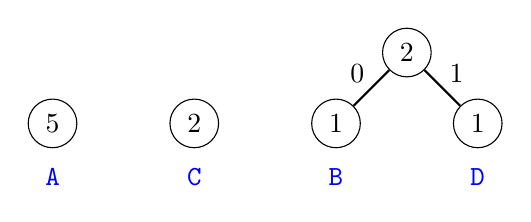
\begin{tikzpicture}[scale=0.9]
\node[draw, circle] (1) at (0,0) {$5$};
\node[draw, circle] (3) at (2,0) {$2$};
\node[draw, circle] (2) at (4,0) {$1$};
\node[draw, circle] (4) at (6,0) {$1$};
\node[draw, circle] (5) at (5,1) {$2$};

\node[color=blue] at (0,-0.75) {\texttt{A}};
\node[color=blue] at (2,-0.75) {\texttt{C}};
\node[color=blue] at (4,-0.75) {\texttt{B}};
\node[color=blue] at (6,-0.75) {\texttt{D}};

\node at (4.3,0.7) {0};
\node at (5.7,0.7) {1};

\path[draw,thick,-] (2) -- (5);
\path[draw,thick,-] (4) -- (5);
\end{tikzpicture}
\end{center}
\begin{comment}
After this, the nodes with weight 2 are combined:
\end{comment}
次に、重さ2の頂点同士を連結する:
\begin{center}
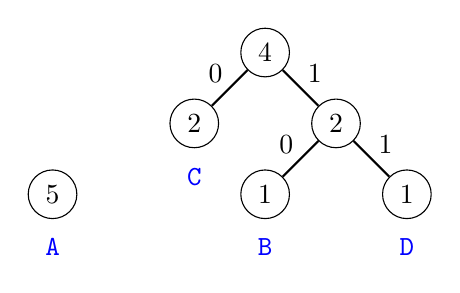
\begin{tikzpicture}[scale=0.9]
\node[draw, circle] (1) at (1,0) {$5$};
\node[draw, circle] (3) at (3,1) {$2$};
\node[draw, circle] (2) at (4,0) {$1$};
\node[draw, circle] (4) at (6,0) {$1$};
\node[draw, circle] (5) at (5,1) {$2$};
\node[draw, circle] (6) at (4,2) {$4$};

\node[color=blue] at (1,-0.75) {\texttt{A}};
\node[color=blue] at (3,1-0.75) {\texttt{C}};
\node[color=blue] at (4,-0.75) {\texttt{B}};
\node[color=blue] at (6,-0.75) {\texttt{D}};

\node at (4.3,0.7) {0};
\node at (5.7,0.7) {1};
\node at (3.3,1.7) {0};
\node at (4.7,1.7) {1};

\path[draw,thick,-] (2) -- (5);
\path[draw,thick,-] (4) -- (5);
\path[draw,thick,-] (3) -- (6);
\path[draw,thick,-] (5) -- (6);
\end{tikzpicture}
\end{center}

\begin{comment}
Finally, the two remaining nodes are combined:
\end{comment}

最後に、残った2つの頂点を連結する:
\begin{center}
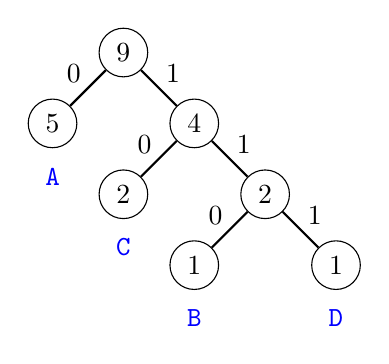
\begin{tikzpicture}[scale=0.9]
\node[draw, circle] (1) at (2,2) {$5$};
\node[draw, circle] (3) at (3,1) {$2$};
\node[draw, circle] (2) at (4,0) {$1$};
\node[draw, circle] (4) at (6,0) {$1$};
\node[draw, circle] (5) at (5,1) {$2$};
\node[draw, circle] (6) at (4,2) {$4$};
\node[draw, circle] (7) at (3,3) {$9$};

\node[color=blue] at (2,2-0.75) {\texttt{A}};
\node[color=blue] at (3,1-0.75) {\texttt{C}};
\node[color=blue] at (4,-0.75) {\texttt{B}};
\node[color=blue] at (6,-0.75) {\texttt{D}};

\node at (4.3,0.7) {0};
\node at (5.7,0.7) {1};
\node at (3.3,1.7) {0};
\node at (4.7,1.7) {1};
\node at (2.3,2.7) {0};
\node at (3.7,2.7) {1};

\path[draw,thick,-] (2) -- (5);
\path[draw,thick,-] (4) -- (5);
\path[draw,thick,-] (3) -- (6);
\path[draw,thick,-] (5) -- (6);
\path[draw,thick,-] (1) -- (7);
\path[draw,thick,-] (6) -- (7);
\end{tikzpicture}
\end{center}

\begin{comment}
Now all nodes are in the tree, so the code is ready.
The following codewords can be read from the tree:
\begin{center}
\begin{tabular}{rr}
character & codeword \\
\hline
\texttt{A} & 0 \\
\texttt{B} & 110 \\
\texttt{C} & 10 \\
\texttt{D} & 111 \\
\end{tabular}
\end{center}
\end{comment}

これで頂点はすべて単一の木を構成し、対応する符号表も完成した。
この木より、以下の符号表が得られる:
\begin{center}
\begin{tabular}{rr}
文字 & 符号 \\
\hline
\texttt{A} & 0 \\
\texttt{B} & 110 \\
\texttt{C} & 10 \\
\texttt{D} & 111 \\
\end{tabular}
\end{center}